\documentclass[a4paper]{report}
\usepackage[utf8]{inputenc}
\usepackage{url}
\usepackage{float}
\restylefloat{figure}
\usepackage{wrapfig}
\usepackage{graphicx}
\usepackage[toc,page]{appendix}
\usepackage{amsmath}
\usepackage{algorithm}
\usepackage[noend]{algpseudocode}
\usepackage[margin=1.0in]{geometry}
\usepackage[colorlinks=true,linkcolor=black,anchorcolor=black,citecolor=black,filecolor=black,menucolor=black,runcolor=black,urlcolor=black]{hyperref}
\usepackage{scrextend}
\graphicspath{ {images/} }
\renewcommand*{\thesection}{\arabic{section}}
\renewcommand{\thesubsection}{\thesection.\alph{subsection}}

\begin{document}
\begin{titlepage}
    \begin{center}
        \includegraphics[width=0.7\textwidth]{uol-logo}

        \vspace{5em}

        \Large{COMP390}
        \vspace{1em}
        \Large{\\2020/21}

        \vspace{3em}

        \Large{LandGAN - Generative Adversarial Networks for Video Game Terrain Generation}

        \vspace{3em}

        \begin{tabular}{|lp{5.0cm}lll|}
            \hline
                                      &                    &  &   & \\
            \textbf{Student Name:}    & Laura Hulley

            \                         &                    &  &     \\
            \textbf{Student ID:}      & 201277571

            \                         &                    &  &     \\
            \textbf{Supervisor Name:} & Prof Paul Dunne

            \                         &                    &  &     \\
            \hline
        \end{tabular}

        \vspace{3em}

        \LARGE{{\textbf{DEPARTMENT OF\\
                        COMPUTER SCIENCE}}}

        \vspace{2em}

        University of Liverpool\\Liverpool L69 3BX

    \end{center}



\end{titlepage}
Thank you to the library group: Henry, Jahan, Rhea and Zakira for their company and valuable advice; and to Izzy and Jenny for making the breaks between studying exciting and unforgettable. As always I am so grateful for my housemates: Amelia, Celine, Hannah, Hannah, Julia, Mollie and Paddy for making lockdown bearable, even enjoyable, and their constant support. Finally, a massive thank you to James and my family, for their endless support and encouragement, and for listening to me talk about elevations and epochs for hours.

\newpage
\begin{center}
\textbf{\Large Generative Adversarial Networks for Terrain Generation}
\vspace{2em}
\end{center}

\begin{figure}[H]
    \centering
        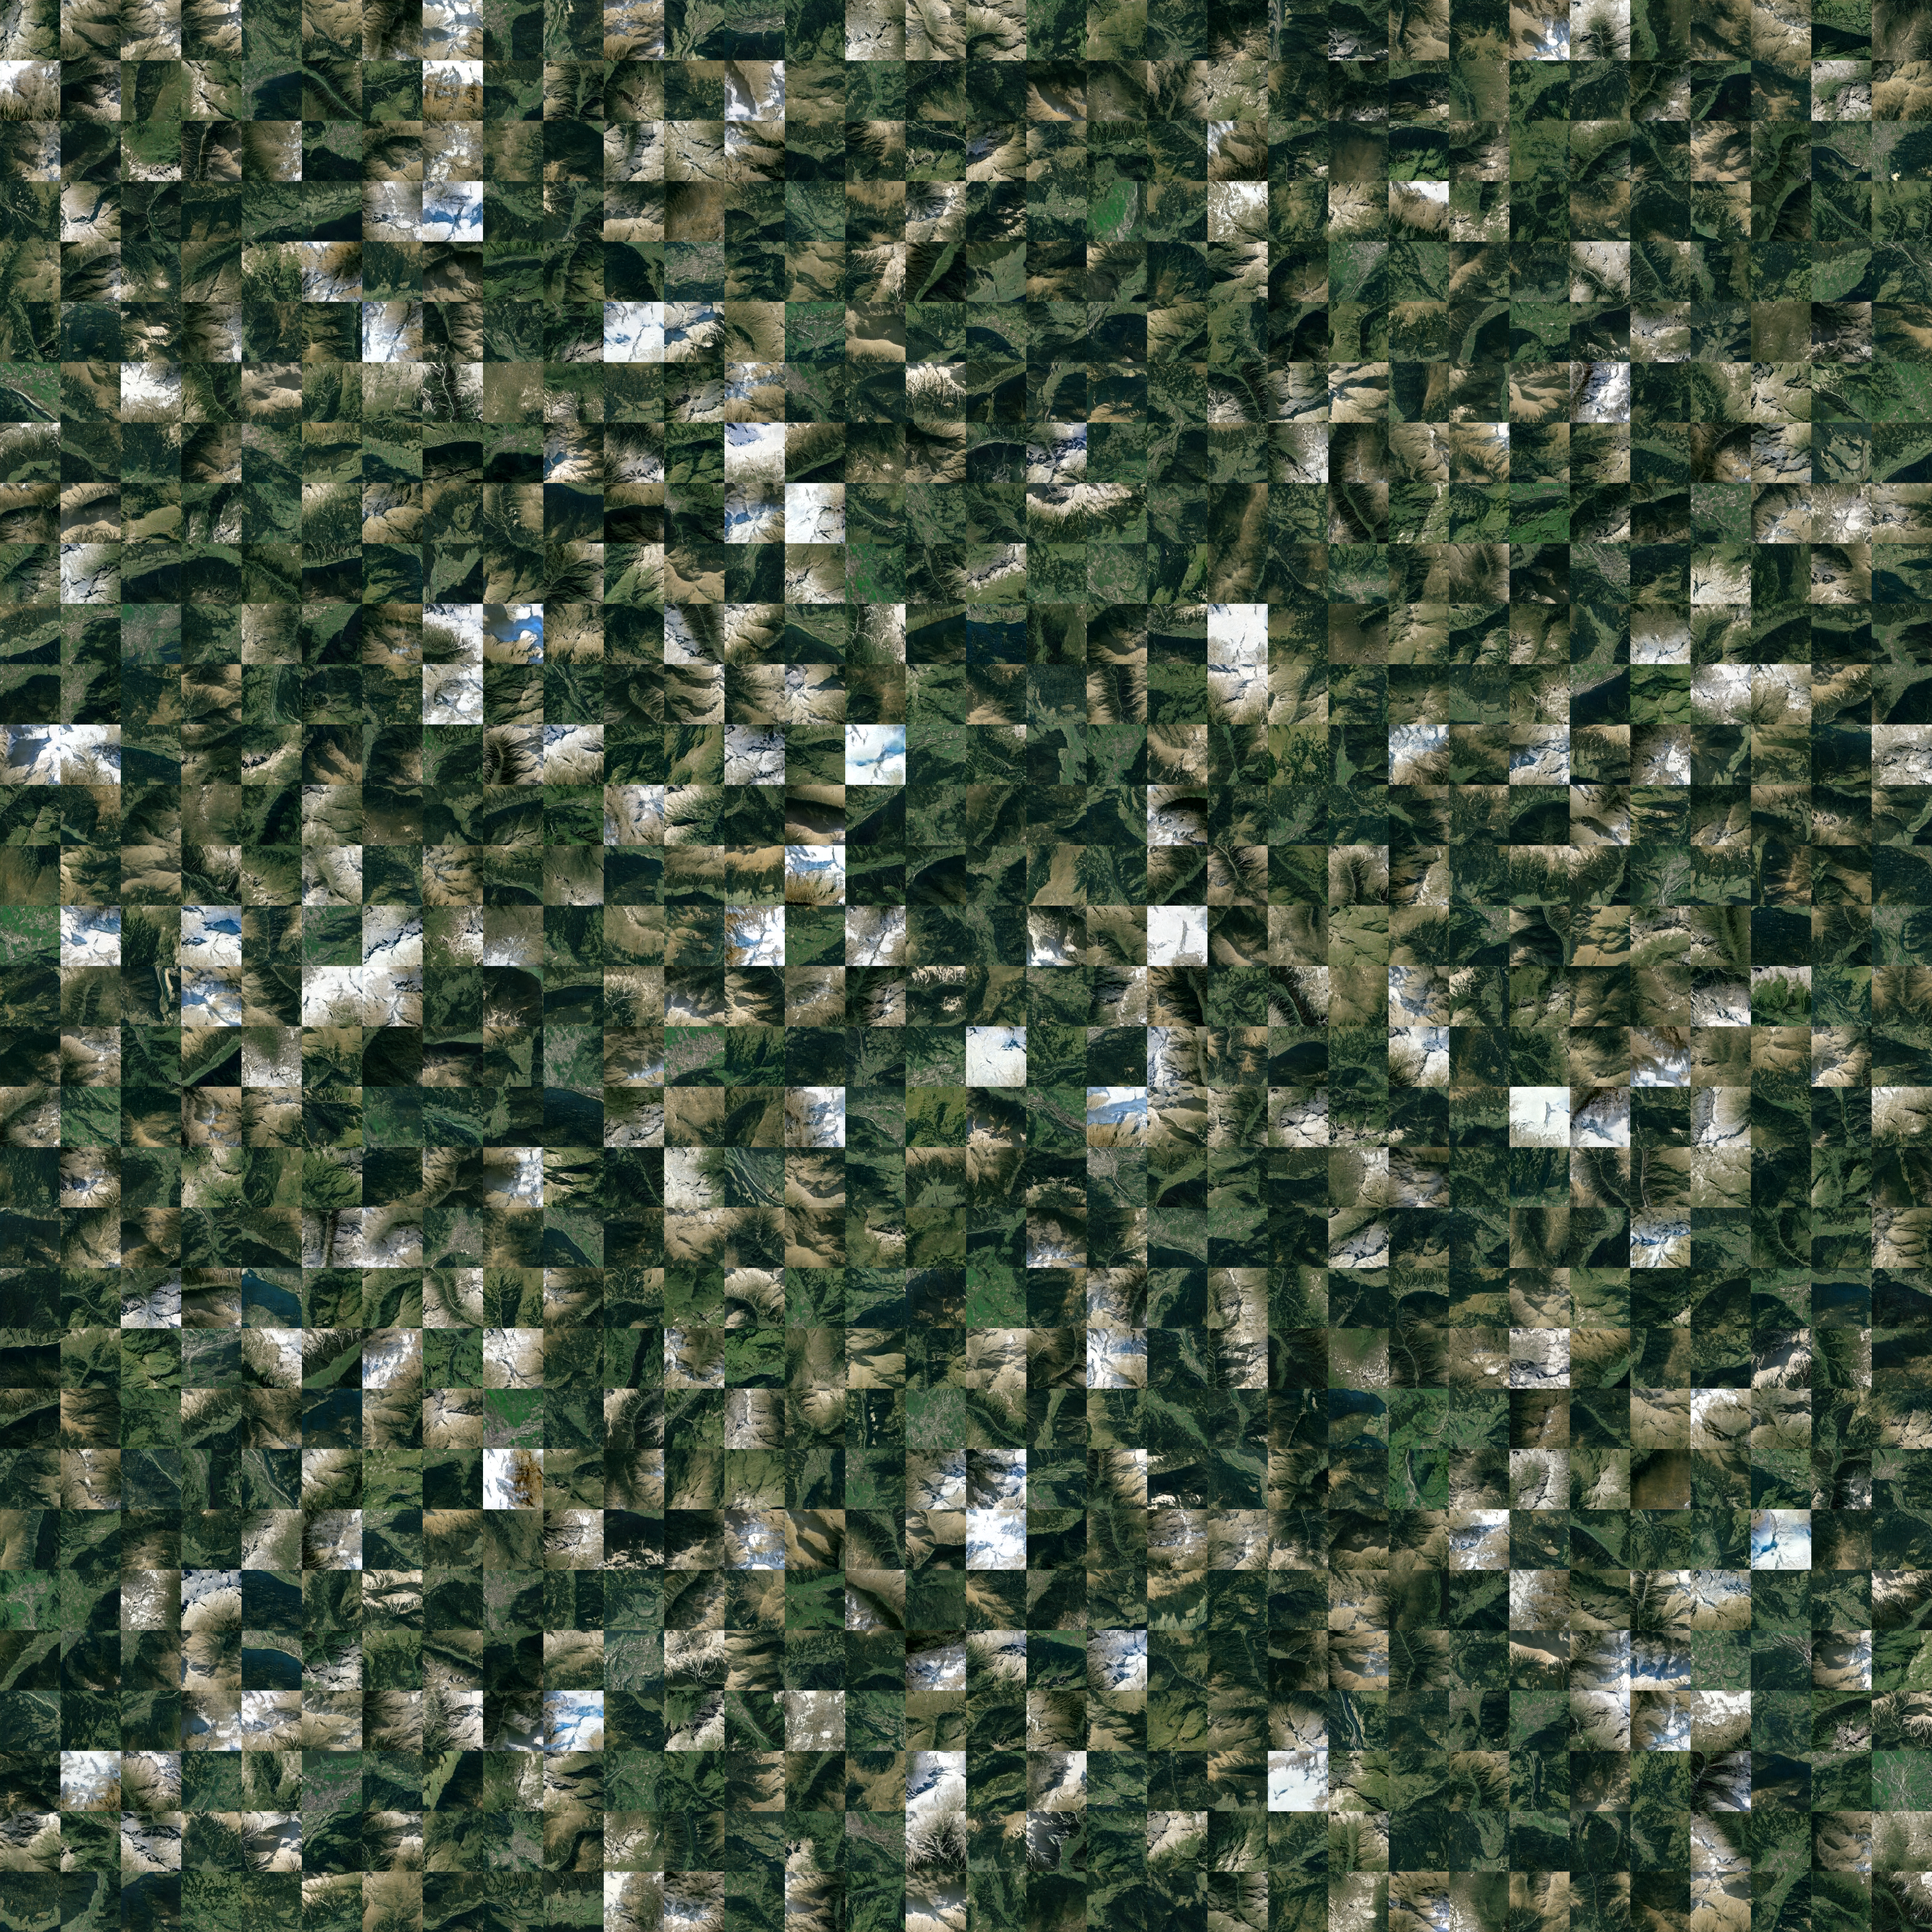
\includegraphics[width=0.75\textwidth]{fakes000800.png}
        \caption{Images generated by StyleGAN2 on a custom-made dataset of satellite imagery}
        \label{fig:title}
\end{figure}

\vspace{1em}

\begin{center}
    \textsc{University of Liverpool, Department of Computer Science}
\end{center}
\begin{center}
    \textsc{COMP390 - 2020/21}
\end{center}

\vspace{3em}

\begin{center}
\textbf{Abstract}
\end{center}
\begin{addmargin}[5em]{5em}
\textit{For decades, procedural terrain generation methods have been based on fractal and noise based techniques. This work proposes that GANs, specifically the StyleGAN architecture, are a suitable alternative method of terrain generation. Multiple datasets are created and used to train a StyleGAN2 model. The results are then displayed as 3D terrains and compared against traditional techniques.}
\end{addmargin}

\newpage
\tableofcontents
\newpage
\section{Introduction}
GANs have been used for a wide variety of applications since their invention in 2014 \cite{goodfellow2014generative}. This project argues the case for the use of GANs, specifically StyleGAN \cite{stylegan}, for terrain generation. The fractal-based `Diamond Square' technique and a noise based method are discussed as methods currently in use today.

Due to a lack of freely available, good quality satellite data online, multiple custom datasets were made. The satellite data was then combined with elevation data to train the model to generate 3D renderings of terrain (figure \ref{fig:intro}). The results of the model are used to compare this technique to traditional techniques, mainly focusing on the Diamond Square algorithm.

\begin{figure}[H]
    \centering
        \includegraphics[width=0.95\textwidth]{intro.png}
        \caption{Images and renders generated by StyleGAN2 on the custom-made dataset of satellite imagery and elevatio}
        \label{fig:intro}
\end{figure}

\subsection{Aims and Objectives}
As outlined in the original proposal (appendix section \ref{appendix:proposal}), this project has two main aims:

\begin{enumerate}
    \item Demonstrate the ability of a GAN to produce realistic and efficient terrain elevation and rendering.
    \item Form a discussion that compares the effectiveness of a GAN technique to more traditional algorithmic techniques.
\end{enumerate}

The first aim is addressed in the following sections, where a GAN is trained on satellite and image data. Other previous studies are also referenced that satisfy this aim.

The second aim, as discussed in the proposal, is more ambiguous. Due lack of readily available quantitative measures for GANs \cite{howgood}, and the time limit of this project, the comparison is based on qualitative measures alone.

\subsection{Background Information}
\subsubsection{Video Game Terrain}
As the video game industry grows, so does the need for more detailed, exciting and extensive terrains. Procedural generation is the main method of generating these terrains and has been an integral part of video games throughout their existence. An early example of such being the entirely ASCII-based 1980 game, Rogue \cite{rogue}. The level maps, treasure, and monsters are procedurally generated each time the game is played. Rogue inspired future games and spawned the category of Rogue-like games which now contains hundreds, if not thousands,\footnote{Figure estimated from Steam search results \cite{roguelikeSteam} and the following list \cite{roguebasin_2020}. There is also the assumption that there are unpublished video games developed using rogue-like techniques.} of procedurally generated games.

The response to the demand for more realistic terrain can be seen in the development of the snowboarding game, SSX(2012) \cite{SSX}. This was the first game in the SSX series to use real world terrain data and the response was overwhelmingly positive. While this was impressive in 2012, it would struggle to compete with the infinite, procedurally generated maps of today's games.

While the terrain in Rogue was formed using simple rule based algorithms, more complex algorithms are needed to create terrain that resembles the natural land forms found on earth. Fractal and noise based techniques can generate incredibly realistic terrain without the limitations of real world data. They offer infinite results and more widely customisable terrain but not without their own drawbacks.

\begin{figure}[H]
    \centering
        \includegraphics[width=0.95\textwidth]{fractals.png}
        \caption{Natural fractals found in the Chinese Himalayas (left) and a romanesco broccoli (right)}
        \label{fig:fractals}
\end{figure}

\paragraph{Fractal Techniques}

Fractals are seen throughout the natural world, from mountains, to rivers, even in broccoli (figure \ref{fig:fractals}). Fractal algorithms are recursive algorithms that preserve self similarity. In nature, an element of randomness is always present and one algorithm that aims to replicate this is the diamond square algorithm (D-Sq).

The D-Sq algorithm begins with a 2d array, the 4 corners of which are set to some initial values. It then iterates between calculating the midpoint of that square, then the midpoints of the resulting `diamonds'. An element of randomness is included in the calculation each time a midpoint is calculated.The values in the resulting array are the `elevation' of the height map and can be plotted in the z axis.

To better understand the algorithm, a simple Python implementation was made which demonstrates the effects of changing the randomness of the algorithm and the resulting `roughness' of the terrain. Figure \ref{fig:fractalPlots} shows the output of the D-Sq script with varying levels of roughness. Two main criticisms of this technique are the presence of artefacts in the resulting terrain and the unrealistic terrain generated (either too regular or too random)\cite{Dsq}. Figure \ref{fig:fractalPlots}(randomness: 5) is an example of the repetitive patterns often generated by this technique. No `mountain' is exactly the same, due to the addition a random value at each iteration, but as a group they can seem unnaturally repetitive. Conversely, with higher levels of roughness or randomness, the mountains can be too steep, sparse and random. Another common problem associated with this technique is the artefacts left behind. Pinches can form between the tiles when the edge values do not line up \cite{proGen}.

\begin{figure}[H]
    \centering
        \includegraphics[width=0.95\textwidth]{fractalPlots.png}
        \caption{Plots produced by the \textit{DSq.py} script at varying levels of roughness. Roughness values used, from left to right: 5, 10, 20, 40.}
        \label{fig:fractalPlots}
\end{figure}

\paragraph{Noise Techniques}

Another common method of terrain generation involves the use of noise. For Perlin noise, `Noise is determined at point (x,y,z) by computing a pseudo-random gradient at each of the eight nearest vertices on the integer cubic lattice and then doing splined interpolation' \cite{perlinN}. The results can be seen in figure \ref{fig:perlin} (left). Compared to real world height maps (figure \ref{fig:perlin}(right)), the limitations of this technique are clearly visible: the patterns produced are far too regular to appear natural.

The merit of both these techniques is that the style of terrain can easily be changed on a large scale. Small changes to the algorithm, such as changing the range of the random inputs, can produce vastly different terrain (as seen previously: figure \ref{fig:fractalPlots}).

\begin{figure}[H]
    \centering
        \includegraphics[width=0.95\textwidth]{perlin.png}
        \caption{Perlin noise (left) and height maps from the Alps dataset used in this project (right).}
        \label{fig:perlin}
\end{figure}

\paragraph{Combined Techniques}
On their own, fractal and noise techniques will only produce a terrain map, with no textures or colouring. To produce a realistic and playable landscape, they must be combined with other algorithms, data or manual input. An example of a software which does just this, is Terragen \cite{terragen}. Decades of development and research into world generation algorithms has resulted in a software that produces incredibly realistic and navigable worlds (figure \ref{fig:terra}). Despite the many complex algorithms and rules used today, the software was originally created using fractal algorithms \cite{Fairc}.

\begin{figure}[H]
    \centering
        \includegraphics[width=0.95\textwidth]{terra.png}
        \caption{Landscapes generated in Terragen}
        \label{fig:terra}
\end{figure}

\subsubsection{Generative Adversarial Networks}
GANs are a relatively recent development in AI. They were first proposed in a 2014 paper by Ian Goodfellow et. al. \cite{goodfellow2014generative}. Since then, GANs have revolutionised generation and creation in a variety of areas; from creating art in the style of Van Gogh \cite{gangogh} to generating faces of people who do not exist\cite{persondoesnotexist}. While the aforementioned approaches seem light-hearted, they showcase the power of GANs to fool even the human eye.

GANs consist of two competitive networks: A generative network and an adversarial network. The adversarial network is trained (in this case) on real world satellite and elevation data and aims to classify whether an input is an example of real satellite imagery and elevation or a fake (produced by the generator).

The aim of the generator is to `fool' the adversarial network into thinking the data it produces has come from the training set. The input to the generator is a vector from a latent space that it applies a function to, to generate the data that can fool the adversarial network. Both networks are trained simultaneously to avoid either network becoming too good at fooling or classifying the other. The adversarial network is trained on how well it classifies real from fake, whereas the generator is trained on how well its results fool the adversarial. A very basic diagram of a GAN is shown in figure \ref{fig:gan}.

\begin{figure}[H]
    \centering
        \includegraphics[width=0.95\textwidth]{generator.png}
        \caption{Simplistic diagram of a general GAN architecture.}
        \label{fig:gan}
\end{figure}

\paragraph{StyleGAN}
In March 2019, NVIDIA released StyleGAN: A Style-Based Generator Architecture for Generative Adversarial Networks \cite{stylegan}. This architecture aimed to demistfy aspects of the image synthesis process within the generator network. Before this, studies largely focused on improving the adversarial network; the generative network was more of a `black-box'. The conclusion from this study was that `the traditional GAN generator architecture is in every way inferior to a style-based design'. A variation on StyleGAN2 \cite{stylegan2} is the specific GAN architecture used for this project. More information on this architecture and the motivations behind this choice are found in sections 1.d and 2.b.

\subsection{Existing work}
\paragraph{Terrain Generation with GANs}
Evidence shows the success of GANs in various aspects of terrain generation. Figure \ref{fig:rivers} shows the results of a PGGAN (progressive GAN) trained on satellite images of US rivers \cite{riverSat}. The success of this study supports the argument for the use of GANs for satellite image generation.

\begin{figure}[H]
    \centering
        \includegraphics[width=0.95\textwidth]{rivers.png}
        \caption{A sample of the results of satellite river generation in \cite{riverSat}}
        \label{fig:rivers}
\end{figure}

As for elevation, a study by Beckham et.al.\cite{beckham2017step} shows similar success generating terrain height maps using NASA elevation data, as seen in Figure \ref{fig:elevs} (left). To texture these height maps, a second generator was used that predicts the colouring for different elevations to varying success (figure \ref{fig:elevs} (right)).

\begin{figure}[H]
    \centering
        \includegraphics[width=0.9\textwidth]{elevs.png}
        \caption{(left) Terrain generated from Nasa elevation data \cite{beckham2017step}. (right) Heightap textures generated by a GAN \cite{beckham2017step}}
        \label{fig:elevs}
\end{figure}

Most closely related to this project is the 2019 paper: `Realistic and Textured Terrain Generation using GANs' \cite{spick}. Spick and Walker use a combination of satellite imagery and elevation data to form 4 channel RGBA images that are then used to train a Spatial GAN (SGAN) \cite{sgan}. The results can be seen in figure \ref{fig:elevGAN}, with further results listed in the appendix at section \ref{appendix:gan}, figure \ref{fig:elevRes}. These show the ability of SGAN to produce relatively accurate results, especially compared to other models such as DCGAN (a deep convolutional GAN). They also show how even SGAN struggles to capture less common features such as sharp ridges and deep valleys. The SGAN results still show a more smoothed out version of the original terrain data. This is one of the failings that this project aims to address with the use of StyleGAN. 

\begin{figure}[H]
    \centering
        \includegraphics[width=0.95\textwidth]{GANelev.png}
        \caption{Sample data generated by an SGAN trained on Nasa satellite and Elevation data. \cite{sgan}}
        \label{fig:elevGAN}
\end{figure}

\subsection{Motivation}
As mentioned previously, the choice of StyleGAN as the architecture for this model was partly due to the `averaging' of the terrain caused by architectures used in previous studies. StyleGAN is an ideal solution for this as the synthesis of the image can be controlled much more precisely. For the Flickr Faces-HQ data set (figure \ref{fig:styles}) this is shown through the ability to control freckles, glasses, hairstyle and other stochastic features. In the case of the terrain data in this project, this can be used to control the presence of features such as snow, mountain peaks, or lakes. In the research for this project there was no work found that utilised StyleGAN for combined satellite imagery and elevation data generation.

\begin{figure}[H]
    \centering
        \includegraphics[width=0.6\textwidth]{styles.png}
        \caption{An example of the stochastic variation possible with the StyleGAN architecture \cite{stylegan}}
        \label{fig:styles}
\end{figure}

The traditional methods of fractal and noise based terrain generation have been used and developed upon for decades. The possibility of using GANs as an alternative or supplement to these methods is the main motivation behind this project. StyleGAN addresses many of the points that fractal and noise techniques struggle with, namely the lack of realism and occurrence of artefacts in the resulting terrains.
\section{Design and Implementation}
\subsection{Dataset Creation}

\subsubsection{Requirements}
\begin{enumerate}
    \item The data set should contain enough data to accurately train a model. At least $\sim$2,500 items.
    \item The script for collecting the data should be easy to adapt to collect data from different regions and zoom levels.
    \item The satellite images used should be an appropriate resolution to the chosen zoom levels, so all features are visible in the image.
    \item The elevation accuracy should be appropriate to the zoom levels used in the satellite images.
    \item The script should combine the satellite images and elevation data into a format that can be encoded to an RGBA PNG file.
\end{enumerate}
\subsubsection{Implementation}
The full script used to fetch the data and encode it to PNG files is stored in the \textit{get\_data.py} file. This script uses the Google Static Maps and Elevation APIs to request the necessary data. Bounding corners of the area to be converted are passed to the script as lat/lng coordinates. The script then iterates through the following loop to convert and save the data as RGBA files.

The process of preparing these files for the model is as follows:
\begin{enumerate}
    \item Select the bounding box of the area to be scanned. For the 128RGBA dataset, an area of the Alps shown in figure \ref{fig:alps} was used, bounded by the coordinates NW:47.309535, 8.968262; SE: 46.098575, 14.054704.
    \item Assign the bounding coordinates values to the variables in the script (lines 1 - 5 in algorithm 1).
    \item Set the zoom level and height/ width of the image (12 and 128*128 respectively for 128RGBA). These variables are used by the API to determine the zoom level and size of the returned image. More information on the input options is available in the API docs \cite{docs}.
    \item The script then requests the image with the Static Maps API and converts it to a tensor (array).
    \item The \textit{elevations} array is then filled with a single request to the Google Elevations API. If the number of pixels in the image is more than the maximum number of requests allowed to the API, the script interpolates the missing values.
    \item The \textit{elevations} array is normalised to a [0,255] range and concatenated with the \textit{image} array.
    \item The resulting tensor is then encoded to an RGBA PNG image and saved.
\end{enumerate}

The pseudocode of the process is shown below.

\begin{algorithm}[H]
    \caption{Initialising variables to request and convert data set}
    \begin{algorithmic}[1]
        \State $areaID\gets$ \text{Location as string} \Comment{For file identification}
        \State $northWestLat\gets$ \text{bounding NW latitude}
        \State $northWestLng\gets$ \text{bounding NW longitude}
        \State $southEastLat\gets$ \text{bounding SE latitude}
        \State $southEastLng\gets$ \text{bounding SE longitude}
        \State
        \State $api\_key\gets$ \text{API key} \Comment{\text{from Google Developer Account}}
        \State $zoom\gets$ \text{Chosen zoom level}
        \State $logoHeight\gets$ \text{Height of google logo on image, in pixels}
        \State $picHeight\gets$ \text{y axis length of requested image, in pixels}
        \State $picWidth\gets$ \text{x axis length}
        \State
        \State $numElevations\gets$ \text{num of elevations to be requested (n*n elevations)}
        \State $elevPoints\gets$ \Call{GetElevPoints()}{}
        \State $minE\gets 80000$ \Comment{Max and min elevation in metres}
        \State $maxE\gets -40$
        \State
        \State $mapHeight\gets 256$ \Comment{\text{Lines 18 - 21 are used for Mercator conversion}}
        \State $mapWidth\gets 256$
        \State $xScale\gets 2^{zoom}/(picWidth/mapWidth)$
        \State $yScale\gets 2^{zoom}/(picHeight/mapHeight)$
        \State
        \State $startLat\gets northWestLat$
        \State $startLng\gets northWestLng$
        \State $startCorners\gets$ \Call{GetImageBounds()}{}
        \State
        \State $lngStep\gets startCorners[3] - startCorners[1]$
        \State
        \State $row\gets 0$
        \State $lat\gets startLat$
        \State
        \While{$lat >= southEastLat$} \Comment{Loop runs until reaches the SW corner of bounds}
        \State $lng\gets startLng$
        \State $col\gets 0$
        \While{$lng <= southEastLng$}
        \If{\Call{CheckIfLand}{lat,lng}$\equiv True$}
        \State $bounds\gets$ \Call{GetImageBounds()}{}
        \State $image\gets$ \Call{RequestImage()}{} \Comment{Request to Google Static Maps API}
        \State $elevSteps\gets$ \Call{GetElevStep()}{}
        \State $elevations\gets$ \Call{RequestElevations()}{} \Comment{Request to Google Elevations API}
        \State \Call{CreateTensor()}{} \Comment{Tensor is saved as a Python pickle file}
        \EndIf
        \State $col\gets col+1$
        \State $lng\gets lng + lngStep$
        \EndWhile
        \State $row\gets row-1$
        \State $lat\gets lat + $ \Call{GetLatStep()}{}
        \EndWhile
    \end{algorithmic}
\end{algorithm}

\subsubsection{Development Environment}
The data set creation script was written in Python, in the VS Code editor. Version control is done with Git and the repository for the script (and all of these files) can be found here \cite{github}. Pipenv is used as a packaging tool to ensure cross compatability of code between systems.

\subsubsection{Design Choices}
\paragraph{File Format - RGBA}
The majority of GAN architectures that were considered for this projected accepted a PNG file as input. A PNG image is typically a 3 channel RBG image: red, green and blue. RGBA is a more uncommon colour format but would work perfectly in this case. The 4th channel, alpha, is used to denote the transparency of the image. For this dataset however, this value is instead used to store the associated elevation data for each pixel. Figure \ref{fig:rgba} shows the structure of each instance in the dataset. The data is formed of 3 dimensional arrays of size (picHeight, picWidth, 4) where pic height and width are the respective size of the image in pixels. Each pixel then has the 4 aforementioned channels associated with it: red, green, blue and alpha (elevation).

There is one main limitation to this format, the values must all be stored as integers. A compromise had to be made to either sacrifice the context of the elevation for the sake of an accurate gradient or vice versa. With a range of -40 to 8,000 metres, it was unlikely the accurate gradients would remain if the values were converted to integers. Because of this, the decision was made to forgo the context of the elevations and instead normalise the elevations from each individual image to a [0,255] range\footnote{This is the range of each of the colour channels of the image. Normalisation to a [-1,1] scale is done as part of the preprocessing of the GAN model.} before casting to integers.

\begin{figure}[H]
    \centering
        \includegraphics[width=0.95\textwidth]{rgba.png}
        \caption{Format of the data in the dataset. Each `pixel' has an associated red, green, blue and alpha value and a lat/lng coordinate can be inferred from its index.}
        \label{fig:rgba}
\end{figure}

\paragraph{Translation From Lat/Lng to Pixel Coordinates}
The Google Static Maps API takes a centre lat/lng as input and outputs a single png image with no accompanying information. One of the biggest obstacles in this project was finding the lat/lng coordinates of the corner of the images in order to request the elevations. There is limited information publicly available about Google's conversion methods but a solution was found using the Mercator projection, as seen in the \textit{PointToLatLng()} and \textit{LatLngToPoint()} functions in the \textit{get\_data.py} file.
The difficulties surrounding this conversion led to the creation of a more general script \cite{tiles}\footnote{\href{https://github.com/hulleylm/google_maps_tiler}{Available \textbf{here}} for easy reference.} for tiling Maps API results, which has been open sourced to avoid others facing the same struggle.

\paragraph{Region Selection}
The alpine region pictured in figure \ref{fig:alps} was chosen for a number of reasons. It was important to generate a similar terrain to that of the examples shown in figures \ref{fig:fractalPlots}, \ref{fig:rivers}, \ref{fig:elevs} and \ref{fig:elevGAN} in order to form a comparison. The fractal property of the terrain also allows us to compare against the fractal technique, without the need for a texture comparison.

The presence of snow in less than half of the images allows an evaluation of the ability of StyleGAN to generate varied data, and not just learn from the averages in the dataset. It can also be used to assess how well the model has learned the correlation between snow and higher elevations.

\begin{figure}[H]
    \centering
        \includegraphics[width=0.95\textwidth]{alps.png}
        \caption{Google Maps satellite view of the area to be scanned}
        \label{fig:alps}
\end{figure}

\paragraph{API Limitations and Array Interpolation}
The majority of limits on the APIs were high enough that they did not affect this project. However, the elevation API only allowed 512 locations per request. $\sim$500 elevation points spread across the image was still within the error margin of Google's elevation data for a 128*128 image. For this reason, the decision was made to find the elevation of an even spread of points across the image and interpolate between these points to form the full array necessary for a complete image. Figure \ref{fig:interpolate} shows the different methods of interpolation tested for the elevation array. `Nearest' uses the nearest available value so the resulting heightmap appears more pixelated. The `Linear' and `Cubic' methods both showed similar results however Linear appeared to smooth out some of the natural ridges so Cubic was chosen instead.

\begin{figure}[H]
    \centering
        \includegraphics[width=0.95\textwidth]{interpolate.png}
        \caption{From left to right: nearest, linear and cubic interpolation methods on the sparse elevation data.}
        \label{fig:interpolate}
\end{figure}

\subsubsection{Evaluation against requirements}
The main dataset used to train the GAN was a set of 2,500 128*128 RGBA PNG images, shown in figure \ref{fig:data}. It took around 2 hours for the script to request, format and save this data. In the run up to this, datasets of different regions, resolutions and zoom levels were created, some of which were tested on the GAN (section 3). The format of the script meant it was easy to change the variables used and the elevation and API requests were automatically reformatted accordingly.

\begin{figure}[H]
    \centering
        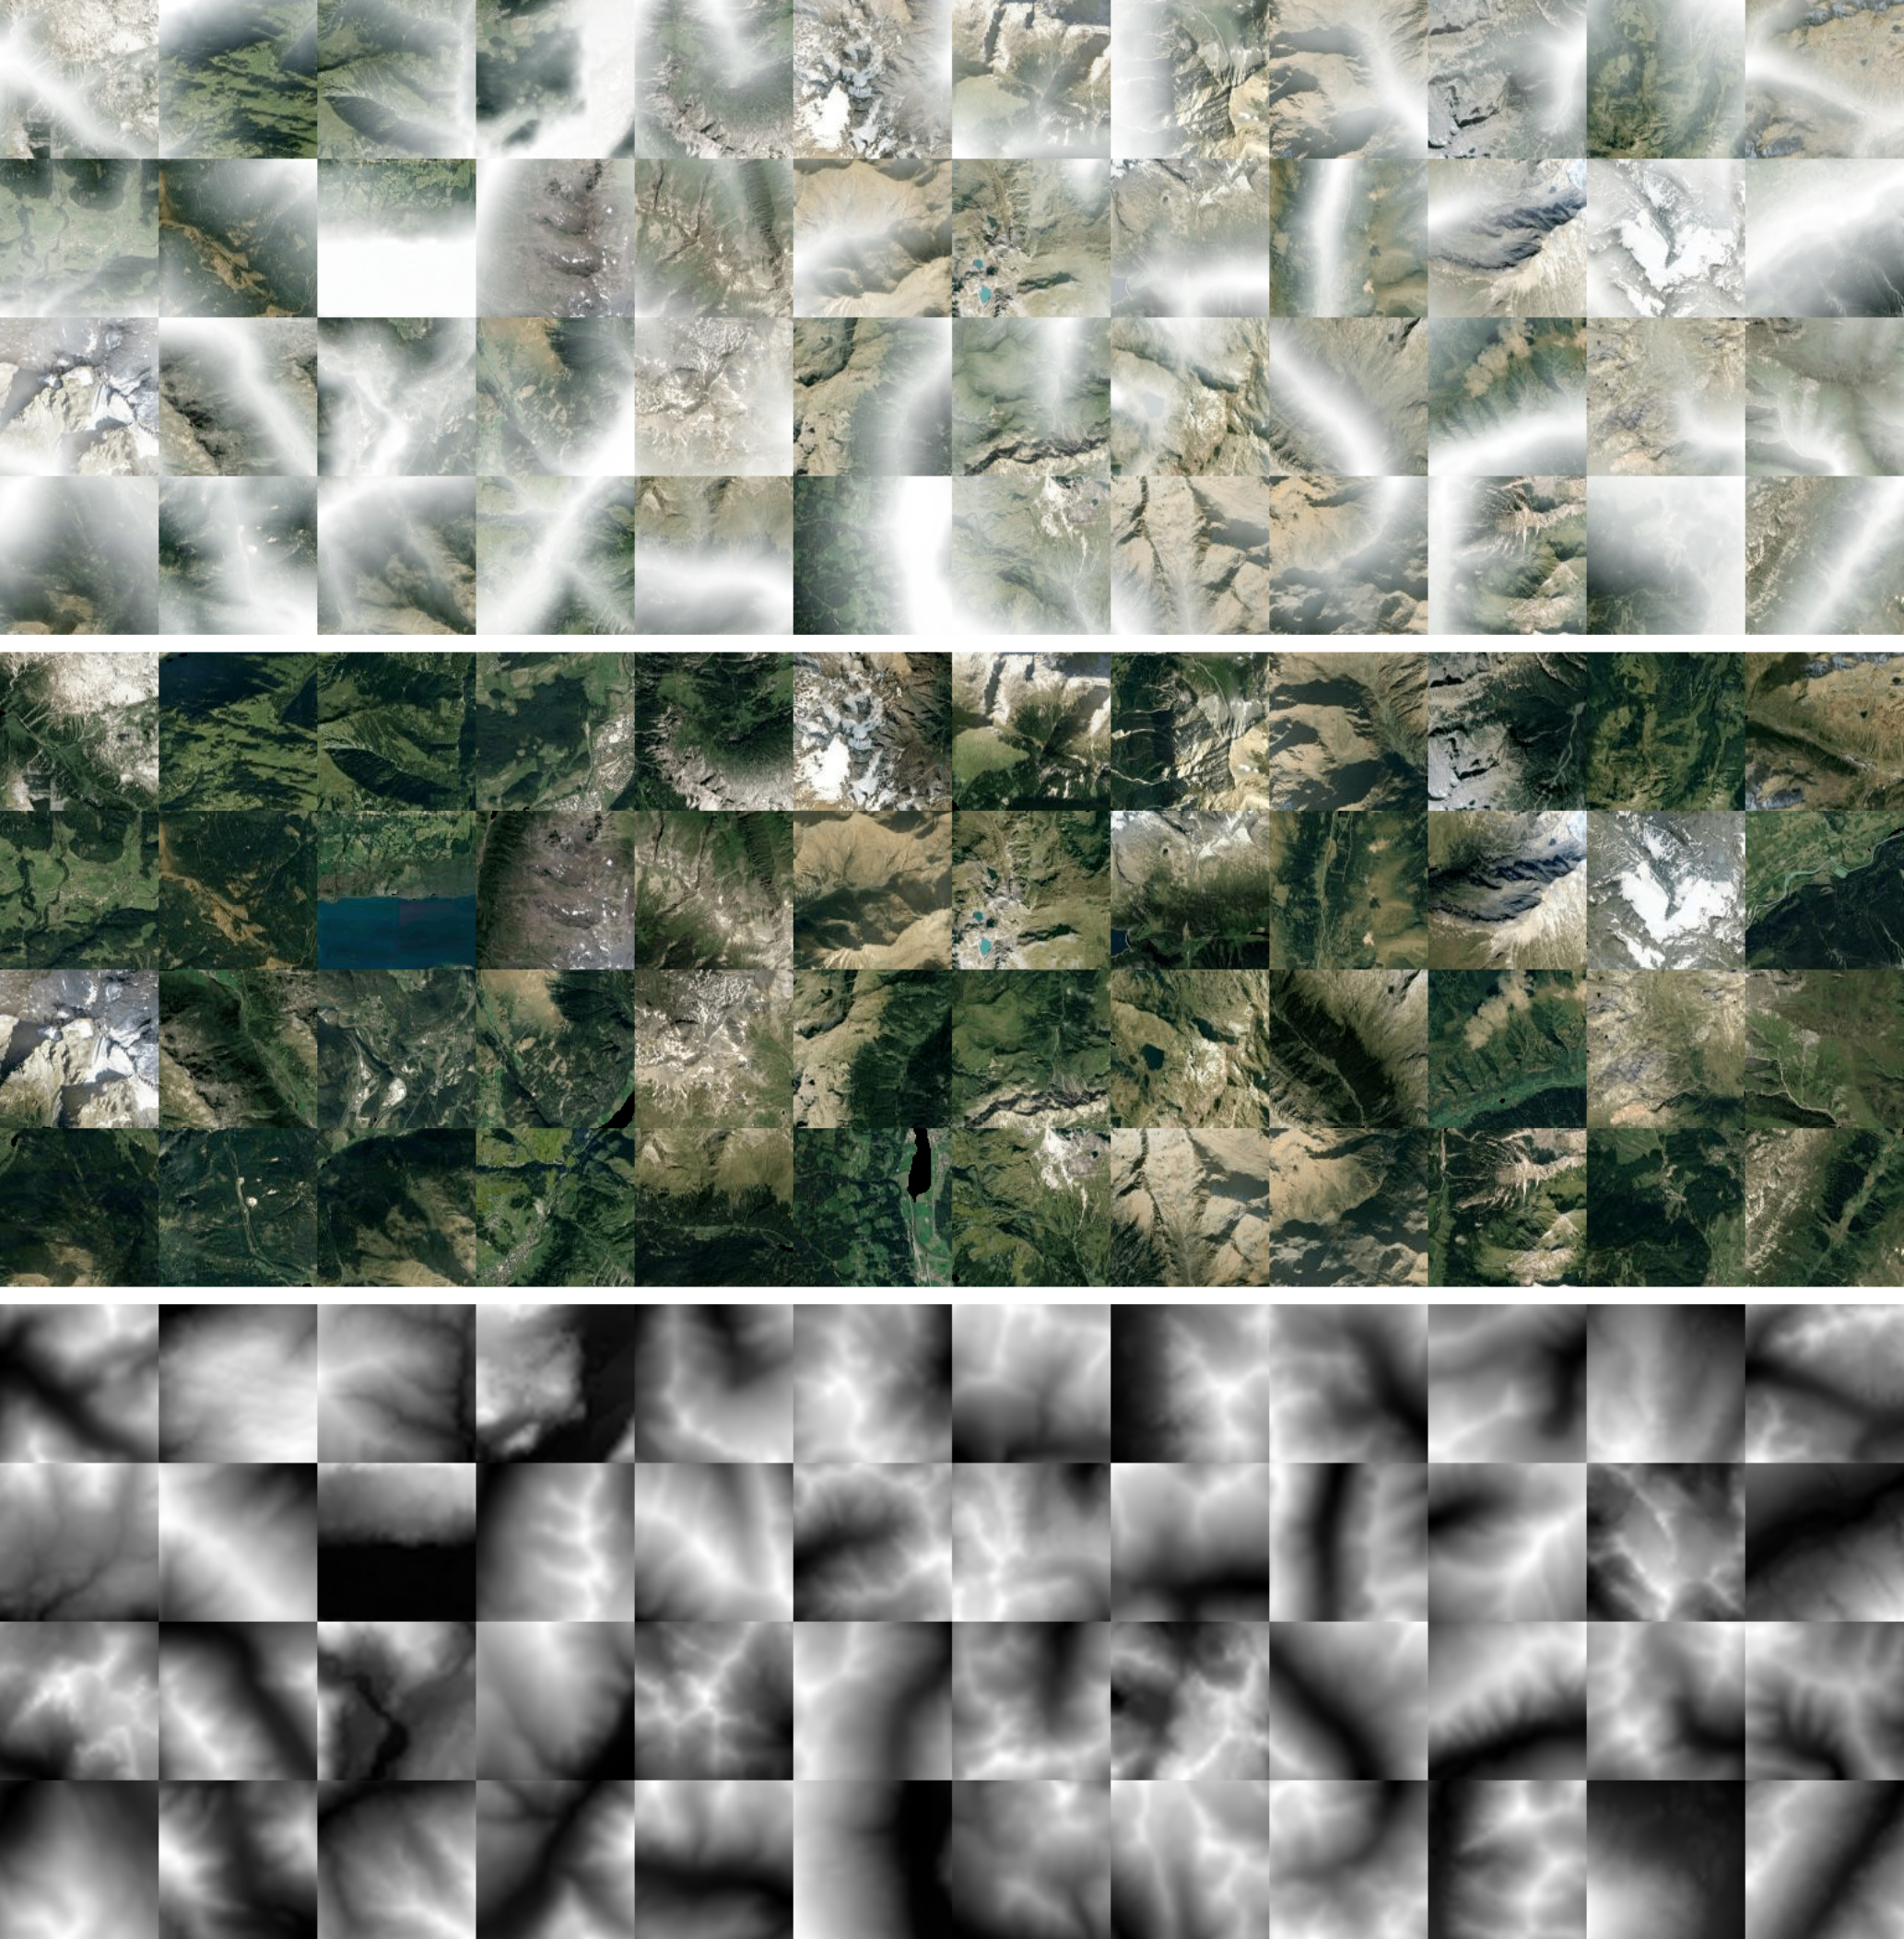
\includegraphics[width=0.95\textwidth]{data.png}
        \caption{The main dataset referenced in this project. From top to bottom: The combined RGBA data (areas of low elevation are transparent and higher elevations are opaque); the first three channels of the data as RGB images; the final channel of the data as greyscale images (height maps)}
        \label{fig:data}
\end{figure}

\subsection{GAN}
\subsubsection{Requirements}
As listed in the original aims of the project, the aim of the GAN was to ideally generate realistic data that is indistinguishable from the data found in the training set. This data should be suitable to form a comparison between GANs and traditional techniques as methods of terrain generation. It was also noted that should this not be possible, a discussion could still be done by referencing previous work on the subject.

\subsubsection{Implementation}
The specific GAN architecture used was a variation of StyleGAN2 \cite{rgbasg}, developed by Vadim Epstein. StyleGAN2 was chosen as the architecture for this project as it has significantly better results than the original model for training on datasets with less that $\sim$30k images. It also boasts faster training, less GPU memory consumption alongside the benefits of the original StyleGAN model mentioned previously (section 1.d). The variation developed by Epstein also added support for 4 channel RGBA images so there were minimal changes to the existing code needed.

\subsubsection{Development Environment}
Initially, it was intended for the code to be run on a personal machine. There were obvious hardware limits with this method and the code was run in a Google Colab notebook instead. Google Pro provides access to a P-100 or V-100 Tesla GPU which enabled quick training times and could be left running in the background. The input dataset, generated images, and snapshots of the model throughout training were all automatically stored on Google Drive, so there was minimal risk of data loss.

\subsubsection{Post-processing}
The data generated by the GAN is in the form of RGBA images. This was the best format for the model but they are not ideal for visualising the resulting terrain. A second script, \textit{split\_images.py} was written that splits the RGBA image into a coloured 3 channel RGB satellite image and a 1 channel greyscale image for the height map. These are then converted to raw files and manually loaded into Unity to model the terrain.

\subsection{Reflections on the development process}
The vast majority of the development time was spent on the creation of the dataset and this is arguably just as important as the development of the GAN. There was no dataset of this format freely available online so constructing this dataset was almost a project in itself. One of the main results presented in the original StyleGAN paper \cite{stylegan} was a new dataset of high quality portrait photos.

A lot of dead ends had to be hit to achieve the software necessary for this project. For the data set development, these are detailed in the `design choices' section. For the GAN, the largest chunk of the time was spent finding an appropriate architecture and setting up the development environment. Originally a lot of time was spent editing the code of StyleGAN2 to accept 4 channel images, before realising that this variation had already been developed.

\section{Testing}
\begin{figure}[H]
    \centering
        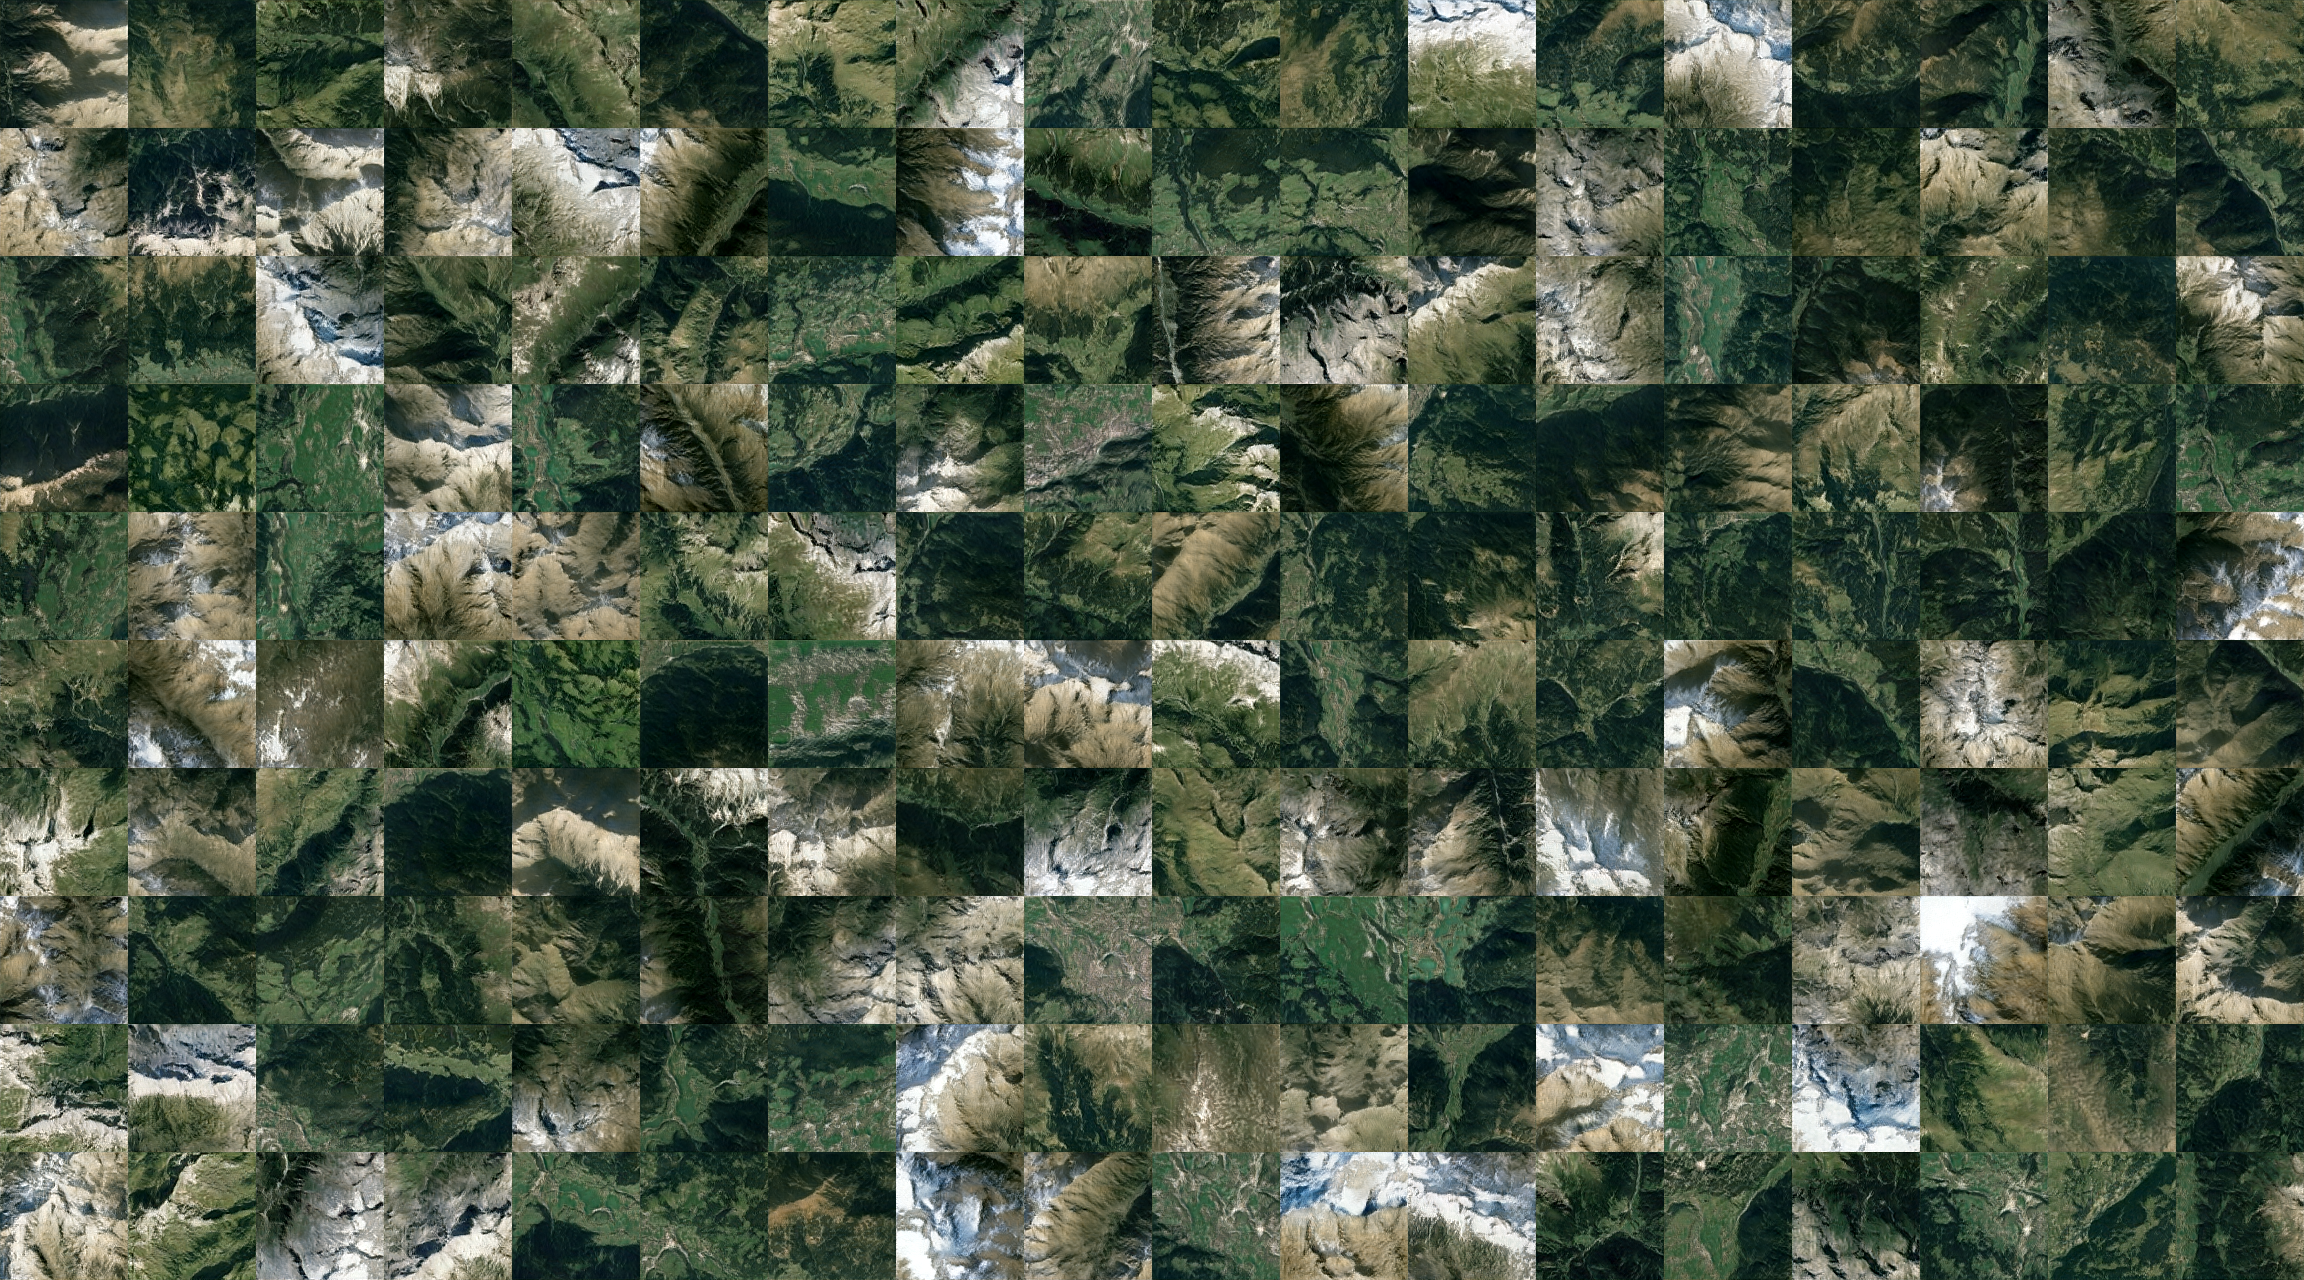
\includegraphics[width=0.95\textwidth]{RGBA128Full.png}
        \caption{An example of terrain data generated by the model.}
        \label{fig:ToDo}
\end{figure}

The GAN model was run on different dataset sizes, resolutions and formats. The resulting data was then converted to animated GIFs, 3D unity models or left as static PNG files. The results of these tests for each dataset are listed below.

\subsection{128*128 RGB Dataset}

This is the easiest dataset to see results as the images are clearly visible to the human eye without the transparency channel. The first run to test the model was done with a dataset of only 50 images and still produced impressive results after 280 epochs \footnote{The seemingly random choice of epochs are largely due to being cut off from the Google GPU. When the WiFi cuts out (which it often does), the training has to be restarted from the most recent save point. This takes time and the results are often already visible by the time it cuts out. For smaller test datasets such as this one, it was not necessary to continue training for many more epochs.}(figure \ref{fig:RGB48}).

\begin{figure}[H]
    \centering
        \includegraphics[width=0.95\textwidth]{RGB48.png}
        \caption{Random samples of data from the original 50 image dataset (left) and the generated data (right).}
        \label{fig:RGB48}
\end{figure}

This confirmed the model would be able to train in a reasonable time on a relatively small dataset. The model was then trained on the finished dataset of 2,500\footnote{The data pre-processing script within the StyleGAN2 code automatically duplicates and mirrors the images. The dataset numbers listed in this section do not account for this, so the model was trained on 5,000 images in this case.} images and trained for 1,200 epochs resulting in figure \ref{fig:RGB2500} as output. \footnote{More outputs and GIF animations of the iterations are available in the GitHub repository for this project: \url{https://github.com/hulleylm/landgan}}

\begin{figure}[H]
    \centering
        \includegraphics[width=0.95\textwidth]{RGB2500.png}
        \caption{A sample of original images from the 128*128 RGB dataset (left) and a sample of images generated by the StyleGAN2 architecture (right).}
        \label{fig:RGB2500}
\end{figure}

\begin{figure}[H]
    \centering
        \includegraphics[width=0.95\textwidth]{RGB128Evo.png}
        \caption{Follows the progression of a vector after increasing epochs. From left to right: 0, 40, 80, 200, 320, 600, 1200 epochs.}
        \label{fig:RGB2500Evo}
\end{figure}

\subsection{128*128 RGBA Dataset}
The RGBA dataset adds the 4th elevation channel to the previous dataset. The images are kept at the same resolution and also trained for 1,200 epochs resulting in the data shown in figure \ref{fig:RGBA128}. The images are much harder to distinguish as the transparency layer converts all the low elevations to a very low opacity. For this reason, the individual image and height map channels are shown in figure \ref{fig:RGBA128Split}. A closer look at some of the images from these samples is seen in figure \ref{fig:RGBA128Ex}.

\begin{figure}[H]
    \centering
        \includegraphics[width=0.95\textwidth]{RGBA128.png}
        \caption{(left) A sample taken from the original dataset of 2,500 128*128 RGBA images. (right) A random sample taken from the images generated by the StyleGAN2 model, trained on the aforementioned dataset}
        \label{fig:RGBA128}
\end{figure}

\begin{figure}[H]
    \centering
        \includegraphics[width=0.95\textwidth]{RGBA128Split.png}
        \caption{The data shown in figure \ref{fig:RGBA128}, split by RGB and elevation channels. Data on the left is from the original dataset and data on the right is a sample of the output of the model.}
        \label{fig:RGBA128Split}
\end{figure}

\begin{figure}[H]
    \centering
        \includegraphics[width=0.95\textwidth]{examples128RGBA.png}
        \caption{A close up of a selection of the generated images shown in figures \ref{fig:RGBA128} and \ref{fig:RGBA128Split}. From left to right: An RGB image that could depict a small town in a valley; an example of some artefacts that can be left by the training process; An RGB image showing well-defined peaks, snow, and shadows; An example of a heightmap exhibiting fractal properties; A combined RGBA image showing ridges as high (opaque) elevation and the valleys between them as low (transparent) elevation.}
        \label{fig:RGBA128Ex}
\end{figure}

GIF animations of the training process were also generated and can be viewed in the \href{https://github.com/hulleylm/landgan}{GitHub \textit{README.md} file}. The 3D terrain models of the results were done using Unity and the results are shown in figures \ref{fig:unity128RGBA} to \ref{fig:contours}.

\begin{figure}[H]
    \centering
        \includegraphics[width=0.95\textwidth]{unity128RGBA.png}
        \caption{An example showing the extra post-processing decisions involved due to the elevations being normalised per-image and losing their context. This figure shows the same instance of generated data (final image in figure \ref{fig:RGBA128Ex}) at two different heights: 300 (left) and 150 (right)}
        \label{fig:unity128RGBA}
\end{figure}

\begin{figure}[H]
    \centering
        \includegraphics[width=0.8\textwidth]{niceUnity.png}
        \caption{3D projection of the centre image in figure \ref{fig:RGBA128Ex}.}
        \label{fig:niceUnity}
\end{figure}

\begin{figure}[H]
    \centering
        \includegraphics[width=0.95\textwidth]{contours.png}
        \caption{A close up view of the contours visible in figure \ref{fig:niceUnity}.}
        \label{fig:contours}
\end{figure}

\subsection{512*512 RGBA Dataset}

Following the success of the 128*128 dataset, a higher resolution dataset was created. The aim of this data was to eliminate the contours visible in the smaller datasets (figure \ref{fig:contours}) and provide an overall better quality rendering. Figures \ref{fig:512Real} to \ref{fig:split} show the images used to train the dataset and a random sample of images generated by the model.

The model took 12 hours to train for 560 epochs. This is significantly longer than the time spent training the smaller dataset for 1,200 epochs and likely due to the increased image resolution.

\begin{figure}[H]
    \centering
        \includegraphics[width=0.95\textwidth]{512realImg.png}
        \caption{Images from the 512*512 RGBA training set, split to show only the first three (RGB) channels. The elevation channel is hidden for the sake of this and the following figure to allow the reader to more accurately compare the generated data to the training set.}
        \label{fig:512Real}
\end{figure}

\begin{figure}[H]
    \centering
        \includegraphics[width=0.95\textwidth]{512RGBfake.png}
        \caption{Data generated by the model, split to show only the first three channels.}
        \label{fig:512Fake}
\end{figure}

\begin{figure}[H]
    \centering
        \includegraphics[width=0.95\textwidth]{512FakeSplit.png}
        \caption{Shows the rightmost image from figure \ref{fig:512Fake}, split into the RGB and elevations channels. From left to right: Original RGBA generated image; RGB image, split from the previous image; the 4th channel of the original generated image, rendered in greyscale as a height map.}
        \label{fig:split}
\end{figure}

\begin{figure}[H]
    \centering
        \includegraphics[width=0.95\textwidth]{512Unity.png}
        \caption{Generated data from figure \ref{fig:split}, modelled as 3D terrain in Unity.}
        \label{fig:512Mountains}
\end{figure}

\begin{figure}[H]
    \centering
        \includegraphics[width=0.95\textwidth]{city.png}
        \caption{Leftmost image from the generated data in figure \ref{fig:512Fake} modelled in Unity.}
        \label{fig:512City}
\end{figure}

Animations of the training process and traversal across vectors can be found in the \href{https://github.com/hulleylm/landgan}{\textit{README.md} file} of this project's \href{https://github.com/hulleylm/landgan}{repo on GitHub}.

\subsection{On Quantitative Testing}
Methods of quantitative testing of GANs have only emerged recently \cite{howgood}. GANs are largely measured by visual inspection. To apply quantitative measures to this project, more flexibility and time would be needed. As such, the methods of evaluating this GAN are almost completely qualitative, bar some mentions of hardware requirements and training time. An obvious improvement to this work would be to measure the Fréchet Inception Distance \cite{FID}, to further evaluate the success of the project.

\section{Evaluation}
Looking at the results from the testing section, it is clear that the model can produce realistic 3D terrain generations. However, there are also some failures and limitations alongside these successes.

\subsection{128*128 RGB Dataset}
This data set was very small compared to any other dataset used but the results (figure \ref{fig:RGB48}) were impressively good. This is likely due to the improved StyleGAN2 model as NVIDIA states that one of the main improvements in this model is the quality of results generated from small datasets. There are a lot of artefacts in the generated images and it is difficult to discern any identifiable features but the colours, gradients, and basic shapes are still present.

The visible success of this small dataset was the deciding factor for this model. It was then trained on a much larger dataset (2,500 images) of the same format. Figure \ref{fig:RGB2500} shows the wide variety of stochastic features it was able to identify and vary between. There are lakes, forests, peaks and snowy areas visible throughout the generated results. The shadows on ridges make sense and the images look realistic from a distance. On much closer inspection, signs of generation are visible. Slightly unnatural curves and patterns on the edges of forests and shadows separate the fake data from the real. This is a very minor feature though and mainly visible when the images are shown in a side-by-side comparison.

\subsection{128*128 RGBA Dataset}
The aim of this project is to generate 3D terrains. This dataset adds the 4th elevation channel but retains the image size and training time (1,200 epochs). The results were similarly impressive to those of the RGB dataset with the added addition of height maps. Modelling the terrain in Unity (figures \ref{fig:unity128RGBA} to \ref{fig:contours}) showed that the model inferred characteristics from the datasets such as sharp ridges, flat valley basins and correctly aligned the elevation and image data.

One main drawback of this and the previous dataset was the low resolution. This was done to allow quick training times (as little as 6 hours for the 1,200 epochs) to quickly see the results of the model. However, this caused contours on the terrain (figure \ref{fig:contours}) and generally very small images. The decision was then made to run the dataset script again to create a higher resolution 512*512 RGBA dataset. The zoom level of the images was also changed to allow for evaluation of the generation of smaller features, such as individual trees, roads and houses.

\subsection{512*512 RGBA Dataset}
Figure \ref{fig:512City} could be interpreted as: a small town, in the base of a valley, with a steep forest-covered hill on one side and a more rocky hill on the other. This is all an assumption of course, as this place is not real. This showcases the ability of the GAN to learn the context of features, in this case the layout of, commonly valley based, alpine towns.

Upon closer inspection, there are elements in the generated data that would make you question their realism. Figure \ref{fig:fakeMistake} (left) could look like houses from a distance, but when compared to houses from the original dataset (figure \ref{fig:realDeal} (left)), you can see the generated houses are less defined and have no geometric shape.

The strange white holes in the landscape in figure \ref{fig:fakeMistake} (right) are not like anything you would expect to see in this landscape. If you compare this to the roads and terrain in figure \ref{fig:realDeal} (right), it seems as though the model has attempted to replicate the winding roads and areas of rock or concrete. Ideally, with more training, the model would better learn how to generate features such as this. At this point it is important to note that this model was only trained for 500 epochs, opposed to the 1,200 epochs on the smaller datasets.

\begin{figure}[H]
    \centering
        \includegraphics[width=0.8\textwidth]{closeFake.png}
        \caption{Close up views of the sample generated data from figure \ref{fig:512Fake}.}
        \label{fig:fakeMistake}
\end{figure}

\begin{figure}[H]
    \centering
        \includegraphics[width=0.8\textwidth]{closeReal.png}
        \caption{Close up views of original data from the training set.}
        \label{fig:realDeal}
\end{figure}

The 3D modelled landscapes generated in figures \ref{fig:512Mountains} and \ref{fig:512City} can now be compared against those generated by Chavdarova et al. \cite{ganTerrain} (figure \ref{fig:elevGAN} and appendices section \ref{appendix:gan}). Figure \ref{fig:GANcompare} clearly shows how the implementation developed as part of this project massively improves upon previous results. There is much more detail and variance in the data generated by StyleGAN2. 

\begin{figure}[H]
    \centering
        \includegraphics[width=0.95\textwidth]{GANcompare.png}
        \caption{(left) Results from \cite{ganTerrain}, (right) Sample 3D terrain generated as part of this project}
        \label{fig:GANcompare}
\end{figure}

\subsection{Comparison Against Traditional Techniques}
The development process of the GAN terrain compared to that of the fractal or noise terrain is very different. The traditional terrains have the obvious advantage of being reproducible on a personal machine, without the need for external GPUs. GANs have a very time, power and memory intensive training process. However once the model has been trained, it is relatively easy and efficient to produce infinite new data. In the context of game development, it is important to consider the compromises that will be made for the sake of efficiency. Often, realism is compromised for the sake of gameplay. However, with the standard of realism expected in games today, it is important to explore new opportunities that could be more efficient than existing techniques.

With all techniques having the possibility of fast and efficient terrain generation (once the GAN has been trained), the question of quality is raised. The data generated in this project exhibits the same fractal properties that the D-Sq algorithm aims to replicate (figure \ref{fig:RGBA128Ex}, fourth left) without the issue of being too random/ regular. Another obvious benefit of the GAN technique is the automatic colouring with an image that is tailored to the terrain.

Extending the GAN terrain to cover a larger area is a complex task, as mentioned in section 4.e. This aspect would need to be developed further in order to accurately compare these techniques for use in an infinite game map.

\subsection{Further Work}
The work presented in this project is by no means complete. It is a proof of concept and intended to be developed upon. Some possible developments and solutions to current limitations are listed below.

\subsubsection{High Performance Computing}
The model is currently run on a 32 core P-100 Tesla GPU. Had there been more time, the code would have been run on the compute nodes of the university's HPC, Barkla. For state-of-the-art results, comparable to those in the original StyleGAN paper (figure \ref{fig:styleres}), NVIDIA advise that the model be trained on NVIDIA DGX-1 with 8 Tesla V100 GPUs.

\begin{figure}[H]
    \centering
        \includegraphics[width=0.95\textwidth]{styleres.png}
        \caption{StyleGAN results from the original paper \cite{stylegan}}
        \label{fig:styleres}
\end{figure}

\subsubsection{Combined Land Cover Data}
Land cover data (as in figure \ref{fig:landCover}) could be used to train a conditional GAN alongside the satellite and/ or elevation data already present. Models such as GauGAN \cite{gauGAN} could allow developers to draw out types of land they would like on their map and have that area automatically elevated and textured by the model. The interactive interface of GauGAN, shown in figure \ref{fig:gauGAN}, shows how a user can define the elements they want in an image and the software can render those elements realistically in a style selected by the user.

\begin{figure}[H]
    \centering
        \includegraphics[width=0.8\textwidth]{copernicus.png}
        \caption{Open source Copernicus land cover data}
        \label{fig:landCover}
\end{figure}

\begin{figure}[H]
    \centering
        \includegraphics[width=0.8\textwidth]{GauGAN.jpg}
        \caption{Interactive user interface for GauGAN \cite{gauGAN}}
        \label{fig:gauGAN}
\end{figure}

Other channels such as climate, population and historical data could also be added to inform rule based algorithms for the game environment. Climate data in particular could be used to control the weather in various regions.

\subsubsection{Infinite terrain}
A GAN can generate infinite numbers of images but the data generated in this project is limited by the image size of the input data. Were the terrains generated to be used for actual gameplay, the user would soon find themselves at the edge of the playable map.

GANs have shown success at predicting and extending existing images \cite{boundless}. Figure \ref{fig:boundless} shows the results of different GAN architectures attempting to extend different images. There is no reason that this technique could not also be applied to the 4channel RGBA images used to train StyleGAN. A second GAN could be used to extend scenes, or even blend together and fill in gaps between generated scenes.

\begin{figure}[H]
    \centering
        \includegraphics[width=0.8\textwidth]{boundless.png}
        \caption{The results of different GAN architectures attempting to extend images. `Ours' refers to the model generated by \cite{boundless}}
        \label{fig:boundless}
\end{figure}

\subsubsection{Customised Results}
StyleGAN is named as such for its ability to control the `style' of the output image. In the case of this project, this ensures variation in the outputs. This is just the beginning. By examining the latent vector space \footnote{For a better understanding of how the latent space affects the specific data for this project, have a look at the GIF in the GitHub repo.} that the data is generated from, you can pin-point the vectors that control certain features, such as glasses (figure \ref{fig:glasses}). The option to customise game terrain could be used by game developers when designing maps but also by the users of the game. Terrains could be more snowy, mountainous or flat but still retain their realism.

\begin{figure}[H]
    \centering
        \includegraphics[width=0.8\textwidth]{glasses.png}
        \caption{Control of stochastic features demonstrated in the original StyleGAN paper. In this case, glasses are `reduced' and removed.}
        \label{fig:glasses}
\end{figure}


\subsubsection{Contextual Elevation Data}
One obvious drawback of using RGBA files as input is the loss of elevation context. Normalising such a large range of elevations to a small scale and converting them to integers would result in a massive loss in accuracy. Adapting the architecture of the GAN model to accept float arrays as input would solve this problem at the cost of the results needing more post-processing to be converted to height maps.

\subsubsection{Higher Resolutions}
Having seen the success of training at a higher resolution, a clear point for progression is the resolution of the images. Google Colab limits GPU usage to 24 hours so there is a limit to what could be achieved easily. There are workarounds however, and the combination of higher resolution images with higher computing power would likely have even better results.

\subsection{Ethical Considerations}
\subsubsection{Data Ownership and Copyright}
The Google terms of service state that anything produced using their APIs must be attributed to them. Google is cited at multiple points in the work so while there is no worry of copyright infringement, it does bring up the larger issue of ownership of GAN-generated data.

The ownership and copyright of data produced by GANs is a heavily debated topic. One such notable copyright issue is the case of the Portrait of Edmond de Belamy \cite{obvious}. This `painting' (figure \ref{fig:obvious}) was generated by a GAN trained on 15,000 images of paintings by various artists over two different time periods. The result sold for \$432,500 at auction but there was heavy criticism about the artwork being available at the Christie's auction in the first place. Critics argued that the `artist', a group called \textit{Obvious}, did not deserve credit for the work.

\begin{figure}[H]
    \centering
        \includegraphics[width=0.5\textwidth]{obvious.jpg}
        \caption{GAN generated artwork - Portrait of Edmond de Belamy}
        \label{fig:obvious}
\end{figure}

The group had only recently started exploring AI for art generation in the past year and the GAN architecture they used had very limited input from them. \textit{Obvious} argued that because they selected the dataset for the model, they deserve credit for the work. None of the members of the groups identified as artists themselves, one was a computer science student and the other two business graduates. A prominent GAN artist, Mario Klingemann compared the artwork to a  `connect the dots children's painting', implying there was no real skill involved on \textit{Obvious}'s behalf.

In terms of this project, it could be argued that no real ownership is deserved here. The data all belongs to Google and the GAN architecture to NVIDIA. It could be argued however, that there is innovation in combining satellite and elevation data to train a GAN, and skill in the process involved. It is unlikely this same feat could be achieved with no significant research and practice in the area.

In any case, with ownership of GAN generated work still heavily contested, this project claims no ownership or copyright on the produced work. All training data is attributed to Google and the majority of the methodology to NVIDIA. The question of ownership of the resulting data is still open for debate. The data generated as part of this project serves only as an argument for the use of GANs for terrain generation. It is unlikely that anything produced using the code given alongside this dissertation could be of any use in commercial work, due to issues listed previously. Should this method or a similar method be employed, permission would need to be granted from Google for the use of their imagery, or at the very least an attribution made.

\subsubsection{Job Replacement}
Since technology's first introductions to the workplace, there have been fears surrounding job loss due to automation. One such example being the introduction of CAD/CAM, which led to fears of many draughtsmen losing their work \cite{cad}.

While Video Game development has always been inherently technology based, there are always manual tasks that can be reduced or made redundant by advancements in technology. With that considered, game developers often use this reduction in manual work as an opportunity to create bigger and better game worlds that would have taken years of work to develop previously. An example of this is Assassin's Creed Unity where designers used city blocks and styles to speed up the process of designing Paris \cite{ign_2014}.

If developing a commercial application of the methods produced in this paper, it is critical to evaluate how it would affect the work of game developers in the industry. The current methods of terrain development should be assessed to ensure the product would enhance the work of developers and not just replace it.

\section{Conclusion}
More research is needed before the terrains generated using the method proposed in this paper can compete with existing traditional methods. Namely, an efficient method of joining or extending the terrain to create an infinite playable area. The processing power and time necessary for training the GAN is another obvious disadvantage of this technique compared to fractal and noise based techniques. However, it must also be taken into consideration that producing infinite new terrains from the GAN, or even training new data on the GAN is already relatively quick and efficient.

The results presented in this dissertation and previous research in the subject offer strong encouragement for further work to be done in this area. The results achieved in a limited time with limited resources are incredibly realistic and pose a real threat to the techniques currently in use today. If these tecniques were to be developed, further research would need to be done into the effect this would have on workers in the industry and any copyright or data ownership issues that may arise surrounding the generation of data.
\section{BCS Project Criteria and Self-Reflection}
\subsection{An ability to apply practical and analytical skills gained during the degree programme}
The fulfilment of this criterion is shown throughout the project. Modules such as \textit{Introduction to Artificial Intelligence} and \textit{Data Mining and Visualisation} taught me the technical background and theory to understand the basics of GANs and machine learning concepts. Throughout my degree I have practised researching skills and have shown this skill in action in section 1.b of this dissertation. Good coding practice has been encouraged and rewarded in many of my modules and enforced the standard of the code produced as part of this project.
\subsection{Innovation and/or creativity}
I chose this project specifically for the opportunity to work on something creative and innovative. As previously mentioned, GANs are a relatively recent development and there is limited research into training them on combined satellite and elevation data. I would argue that having found only one other paper that follows a similar approach, the idea itself is innovative. 
\subsection{Synthesis of information, ideas and practices, to provide a quality solution together with an evaluation of that solution}
This is evidenced in all previous sections of the dissertation and project. Previous work in the area was researched and discussed, then used to inform the development of the project. The software was then tested, and the results evaluated, to come to a conclusion on the project.
\subsection{Project meets a real need in a wider context}
Innovation is important in all aspects of computer science. This project directly addresses needs in the context of video games but could also be used in other areas such as virtual terrains for simulations.
\subsection{Ability to self-manage a significant piece of work}
This project was all managed by me with limited input of others. I stuck to the initial timescales I laid out in my proposal until an unexpected amount of deadlines came at once and I was forced to postpone. I worked on the project regularly throughout the year (as evidenced by my GitHub commits).

With no previous experience in GANs, I taught myself the theory behind them enough to tailor a dataset for use with one myself. Before beginning this project I had no experience in Latex, Git or Unity so these were all self taught alongside my studies.
\subsection{Critical self-evaluation of the process}
There is an obvious over-simplification of some aspects of this project. The inner workings of the GAN are left relatively unchanged or explained and a very simplistic version of the traditional fractal and noise techniques are discussed. To fully explore this topic I would have needed much more time and ideally some more experience in the area. I believe the amount of detail covered in this dissertation is sufficient for an undergraduate project, but ideally I would have liked to spend more time doing quantitative measurements of the model or even adapting the architecture more to my use case.

This has undoubtedly been one of the most exciting and interesting parts of my degree and I was surprised with the quality of results I was able to produce. Having limited experience writing work of this style, I found I underestimated the time it would take to collect all of my research together and discuss my findings. A very busy late April/ early May meant I had to prioritise my module coursework and delay the deadline for the dissertation. In hindsight, I should have started the implementation of the GAN a lot earlier and spent less time fine-tuning and refactoring my dataset collection script.

Overall my experience working on this project has been overwhelmingly positive. I have had the chance to use new, state-of-the-art algorithms to produce work that I have found no evidence of being done before. My coding skills have improved, especially in terms of producing code that is sustainable and user-friendly. Alongside this project I read the book `Clean Code in Python' \cite{clean} which taught me a lot and ensured my code was of a good standard and easily reusable by others via GitHub, for the exploration of similar projects.
\renewcommand\bibname{References}
\bibliographystyle{IEEEtran}
\bibliography{refs}
\begin{appendices}
\section{Aims and Objectives, as taken from the proposal}
\label{appendix:proposal}
\subsection{Aims}
\begin{enumerate}
    \item Demonstrate the ability of a GAN to produce realistic and efficient terrain elevation and rendering.
    \item Form a discussion that compares the effectiveness of a GAN technique to more traditional algorithmic techniques.
\end{enumerate}
\subsection{Objectives}
\subsubsection{Aim 1}
\begin{enumerate}
\renewcommand{\theenumi}{\alph{enumi}}
    \item Source satellite image and elevation data of the planet that is legally available for educational use.
    \item Source a sufficient amount of training data for the GAN to enable a fair comparison. The definition of a sufficient amount of training data for the discriminator would need to be defined in later stages of the project after initially testing the success of the model.
    \item Define a measure of success for the GAN.
    \item Develop a GAN with the aim of producing results that are indistinguishable by humans from those in the original data set. This objective is a desirable requirement of the model developed, however the closer the model is to reaching this standard, the better we are able to argue the merits of this approach. The process of developing a GAN will also increase my personal understanding of the subject and allow a more informed discussion.
\end{enumerate}
\subsubsection{Aim 2}
\begin{enumerate}
    \renewcommand{\theenumi}{\alph{enumi}}
    \item Outline the main similarities and differences between the use of GANs and traditional approaches to terrain generation.
    \item Form a meaningful argument. As this project is an investigation into how one technique compares to another, there is no bias to have a definite `winner'. To be classified as a meaningful argument, in line with the aforementioned article, this objective would be satisfied by completion of objectives c-e.
    \item Frame of reference: Define the context in which these techniques are being measured. For example, in the intended context of game design, it is worth noting why we would place more weight on the efficiency of the program at the expense of realism.
    \item Grounds for comparison: Explain the rationale behind the choice of terrain generation techniques used as examples in the project.
    \item Clearly define the relationship between the techniques: "Do they extend, corroborate, complicate, contradict, correct, or debate one another?"
    \end{enumerate}
\section{Spick and Walker: GAN Terrain}
\label{appendix:gan}
    \begin{figure}[H]
        \centering
            \includegraphics[width=0.9\textwidth]{evelRes.png}
            \caption{Shows the results of satellite river generation in \cite{riverSat}}
            \label{fig:elevRes}
    \end{figure}
\section{Code}
Code here?
\end{appendices}
\end{document}